\documentclass[a4paper,11pt]{article}
\usepackage{geometry}
\usepackage[T1]{fontenc}
\usepackage[utf8]{inputenc}
\usepackage{lmodern}
\usepackage[francais]{babel}
\usepackage{authblk}
\usepackage{tabularx}
\usepackage{longtable}
\usepackage{array}
\usepackage{listings}
\usepackage{color}
\usepackage{float}
\usepackage{graphicx}


\begin{document}

\begin{titlepage}
  \newcommand{\HRule}{\rule{\linewidth}{0.5mm}} % Defines a new command for the horizontal lines, change thickness here

  \center % Center everything on the page
   
  %----------------------------------------------------------------------------------------
  %	HEADING SECTIONS
  %----------------------------------------------------------------------------------------

  \textsc{\LARGE INSA de Lyon}\\[1.5cm] % Name of your university/college
  \textsc{\Large DASI}\\[0.5cm] % Major heading such as course name
  \textsc{\large Collect'IF : partie 1}\\[0.5cm] % Minor heading such as course title

  %----------------------------------------------------------------------------------------
  %	TITLE SECTION
  %----------------------------------------------------------------------------------------

  \HRule \\[0.4cm]
  { \huge \bfseries Dossier d'analyse}\\[0.1cm] % Title of your document
  \HRule \\[1.5cm]
   
  %----------------------------------------------------------------------------------------
  %	AUTHOR SECTION
  %----------------------------------------------------------------------------------------

  % If you don't want a supervisor, uncomment the two lines below and remove the section above
  \Large \emph{Auteurs:}\\[1cm]
  \newcolumntype{R}{>{\raggedleft\arraybackslash}X}
  \newcolumntype{L}{>{\raggedright\arraybackslash}X}
  \begin{table}[h]
    \begin{center}
      \begin{tabularx}{10cm}{R L}
         Pierre-louis & \textsc{Lefebvre} \\
         Nicolas & \textsc{Six} \\[5cm]
      \end{tabularx}
    \end{center}
  \end{table}
  
  %----------------------------------------------------------------------------------------
  %	DATE SECTION
  %----------------------------------------------------------------------------------------

  {\large \today}\\[3cm] % Date, change the \today to a set date if you want to be precise

  %----------------------------------------------------------------------------------------
  %	LOGO SECTION
  %----------------------------------------------------------------------------------------

  %\includegraphics{Logo}\\[1cm] % Include a department/university logo - this will require the graphicx package
   
  %----------------------------------------------------------------------------------------

  \vfill % Fill the rest of the page with whitespace

\end{titlepage}
\tableofcontents
\pagebreak

%end header

\section{Modèle du domaine}

\begin{figure}[h]
  \begin{center}
    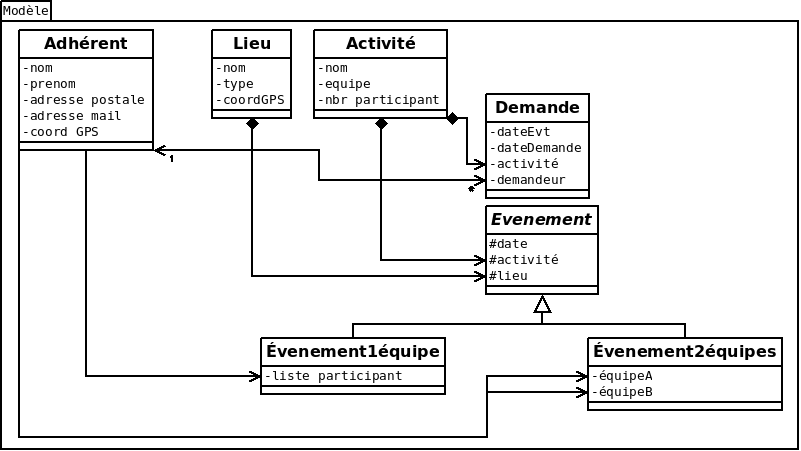
\includegraphics[width=15cm]{../modèle.png}
    \caption{Modèle du domaine}
  \end{center}
\end{figure}

\section{Description des services}

\paragraph{}
Affin d'assurer le bon fonctionnement de l'aplication nous avons dénombrer un certain nombre de services nécésaire à l'aplication. Ces services sont rassembler ci-desous sous forme d'un tableau reprenant les éléments présent dans la JavaDoc.

\newcolumntype{P}[1]{>{\raggedright}p{#1}}

\begin{table}[H]
  \begin{center}
    \caption{ServicesMetier.java}
    \label{tab:ServicesMetier}
    \begin{longtable}{|P{7cm}|p{7cm}|}
      \hline
       void affecterLieuAEvenement(Lieu lieu, Evenement evenement) & Affecte un lieu a un evenement et envoye le mail correspondant \\ \hline
       List<Demande> afficherDemandesTrierParActiviteeDesc() & Renvoie la liste des demandes contenue dans la base de donnee, trier par nom d'activitee decroissant  \\ \hline
       List<Demande> afficherDemandesTrierParDateDescPourAdherent(Adherent adherent) & Renvoie la liste des demandes de l'adherent donnee en parametre, trier par ordre de date decroisante  \\ \hline
       void creerActivite(Activite activite) & Methode permettant d'ajouter une activite a la base  \\ \hline
       int creerAdherent(Adherent adherent) & Methode permettant d'ajouter un adherent a la base, seulement si celui-ci identife par son adresse mail n'existe pas deja dans la base de donne, gere aussi l'envoi des mails d'infirmation ou de confirmation d'inscription  \\ \hline
       void creerDemande(Demande demande) & Ajoute a la base de donnee une demande  \\ \hline
       void creerEvenement(Evenement evenement) & Ajoute a la base de donnee un evenement  \\ \hline
       void creerLieu(Lieu lieu) & Methode permettant d'ajouter un lieu a la base  \\ \hline
       List<Activite> obtenirActivitees() & Renvoie la liste complete des activitees presante dans la base de donnee  \\ \hline
       List<Demande> obtenirDemandesTrierParActivitee() & Renvoie la liste des demandes contenue dans la base de donnee, trier par nom d'activitee croissant  \\ \hline
       List<Demande> obtenirDemandesTrierParDatePourAdherent(Adherent adherent) & Renvoie la liste des demandes de l'adherent donnee en parametre, trier par ordre de date croisante  \\ \hline
       List<Evenement> obtenirEvenementSansLieu() & Methode renvoye une liste de tous les evenements affectes a aucun lieu  \\ \hline
       List<Lieu> obtenirLieux() & Renvoie la liste des Lieux contenue dans la base de donnee  \\ \hline
       Evenement rechercherEtCreerEvenement(Activite activite, java.util.Date date) & Renvoie l'evenement creer si la creation a eu lieu, null sinon  \\ \hline
       Activite trouverActivite(java.lang.String nom) & Renvoie l'activite corespondant au nom fournie  \\ \hline
       Adherent trouverAdherent(long id) & Renvoie l'adherent corespondant a l'ID fournie  \\ \hline
       Adherent trouverAdherent(java.lang.String mail) & Renvoie l'adherent corespondant au mail fournie  \\ \hline
       Evenement trouverEvenement(long id) & Renvoie l'evenemnt corespondant a l'ID fournie  \\ \hline
       Lieu trouverLieu(long id) & Renvoie le lieu corespondant a l'ID fournie \\ \hline
    \end{longtable}
  \end{center}
\end{table}

\begin{table}[H]
  \caption{ServiceTechnique.java}
  \label{tab:ServiceTechnique}

  \begin{center}
    \begin{tabular}{|P{7cm}|p{7cm}|}
    \hline
       static void mailConfirmationInscriptionAdherent(Adherent adherent) & Affiche sur la console le mail que l'adherent reçoit en cas de confirmation de son inscription \\ \hline
       static void mailConfirmationInscriptionResponsable(Adherent adherent) & Affiche sur la console le mail que le responsable recoit en cas de confirmation de l'inscription d'un adherent passe en parametre \\ \hline
       static void mailEvenement(Evenement evenement) & Affiche sur la console le mail que le responsable envoie en cas de creation d'un evenement passe en parametre \\ \hline
static void mailInfirmationInscriptionAdherent(Adherent adherent) & Affiche sur la console le mail que l'adherent recoit en cas d'infirmation de son inscription \\ \hline
static void mailInfirmationInscriptionResponsable(Adherent adherent) & Affiche sur la console le mail que le responsable recoit en cas d'infirmation de l'inscription d'un adherent passe en parametre \\ \hline
static void majCoordonnees(Adherent adherent) & Methode de mise a jour de la latitude et longitude d'un Adherent \\ \hline
static void majCoordonnees(Lieu lieu) & Methode de mise a jour de la latitude et longitude d'un Lieu \\ \hline
    \end{tabular}
  \end{center}
\end{table}


\pagebreak
\section{Maquette des IHMs}

\subsection{IHM Utilisateur}

\subsubsection{Schema générale}

\paragraph{}
L'interface utilisateur est composé de deux vues distinctes: une vues de connexion et une d'utilisation. La première est décliné en quatre variente différente en fonction des informations à afficher sur la page.

Les différents liens entre ces interfaces graphiques sont explicitée sur la Figure~\ref{IHMs} qui représente les différent cas d'utilisation de la vu de connexion. Il est important de préciser que même avec l'affichage d'un message d'erreur ou de confirmation la vu de connexion est toujours utilisable et se comporte comme une vue de connexion normale. De plus comme il le sera expliqué plus tard il est possible de revenir à la vu de connexion une fois sur la vu d'utilisation en utilisant le bouton "déconexion".

\begin{figure}[H]
  \begin{center}
    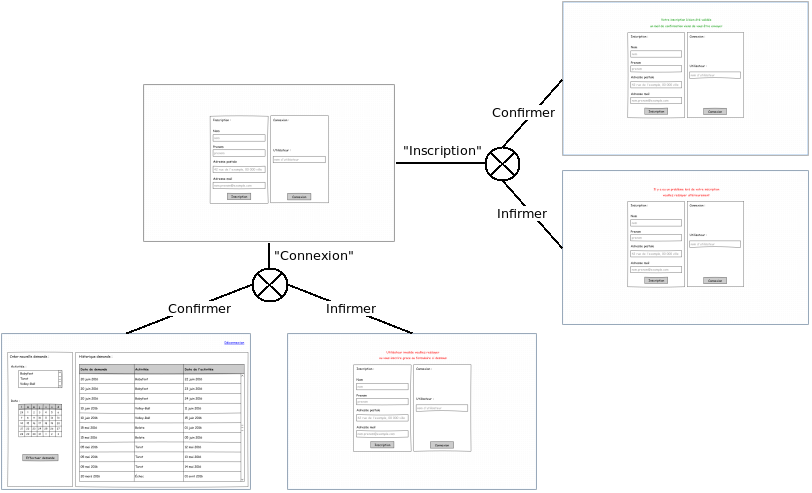
\includegraphics[width=15cm]{../../IHM/graphique_IHM.png}
    \caption{Mises en relation des IHMs}
    \label{IHMs}
  \end{center}
\end{figure}
\pagebreak
\subsubsection{IHM de connexion du client}

\paragraph{}
Cette IHM permet à l'Utilisateur de se connecter à COllect'IF par simple saisie de sont adresse mail dans le menu de conection de la colonne de droite ou dans le cas où celui-ci ne posède pas encore de compte de s'en crée un graçe au menu d'inscription de la colonne de gauche.

\begin{figure}[H]
  \begin{center}
    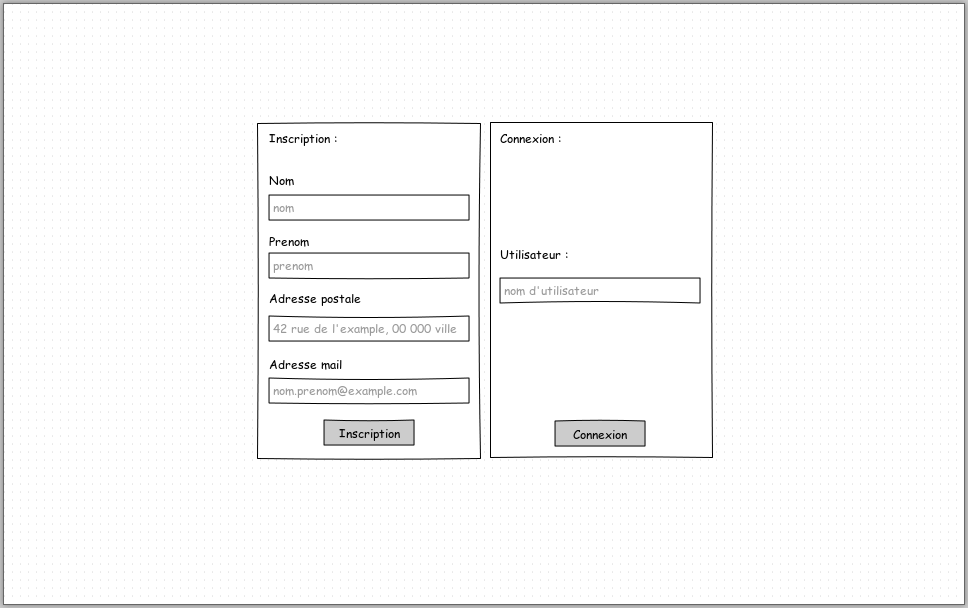
\includegraphics[width=15cm]{../../IHM/IHM_connection_utilisateur.png}
    \caption{IHM de connexion du client}
  \end{center}
\end{figure}

\paragraph{}
Comme expliquer plus haut et ilustrer dans la Figure~\ref{IHMs}, en fontion de l'action éffectué ainsi que des données saisie différents messages de confirmation ou d'erreur peuvent être affiché. Des illustration de ces différent mesages vous sont proposé ci desous.

\begin{figure}[H]
  \begin{center}
    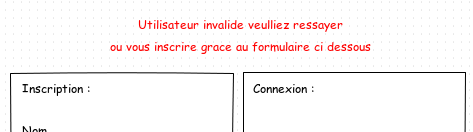
\includegraphics[width=15cm]{../../IHM/IHM_connection_utilisateur_erreur_co_z.png}
    \caption{IHM erreur de connexion du client}
  \end{center}
\end{figure}

\begin{figure}[H]
  \begin{center}
    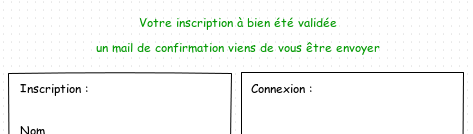
\includegraphics[width=15cm]{../../IHM/IHM_connection_utilisateur_conf_ins_z.png}
    \caption{IHM confirmation d'inscription}
  \end{center}
\end{figure}

\begin{figure}[H]
  \begin{center}
    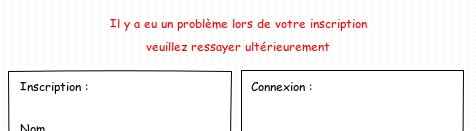
\includegraphics[width=15cm]{../../IHM/IHM_connection_utilisateur_erreur_ins_z.png}
    \caption{IHM erreur d'inscription}
  \end{center}
\end{figure}

\pagebreak
\subsubsection{IHM utilisateur connecté}

\paragraph{}
L'IHM de l'utilisateur est décomposé en deux colonnes. La première sert à créer une nouvelle demande d'évènement. Affin de l'aider dans cette tâche l'utilisateur à accès à une liste des activitées possibles dans laquel il peut trouver facilement ce qu'il recherche en entrant la première lettre du nom de l'activiée qu'il souhaite. De plus graçe à une vue de type calendrier il peut choisir le jour où il voudrait évectuer cette activitée.

La segonde colonne affiche l'historique des demandes de l'utilisateur comprenant la date de demande, le type d'activitée demandé ainsi que la date choisie pour l'évènement, trier par date de demande.

Un boutons de déconnexion est aussi proposé à l'utilisateur, ce lien lui permet de cloturer sa séssion et de revenir simplement sur la page de connexion.

\begin{figure}[H]
  \begin{center}
    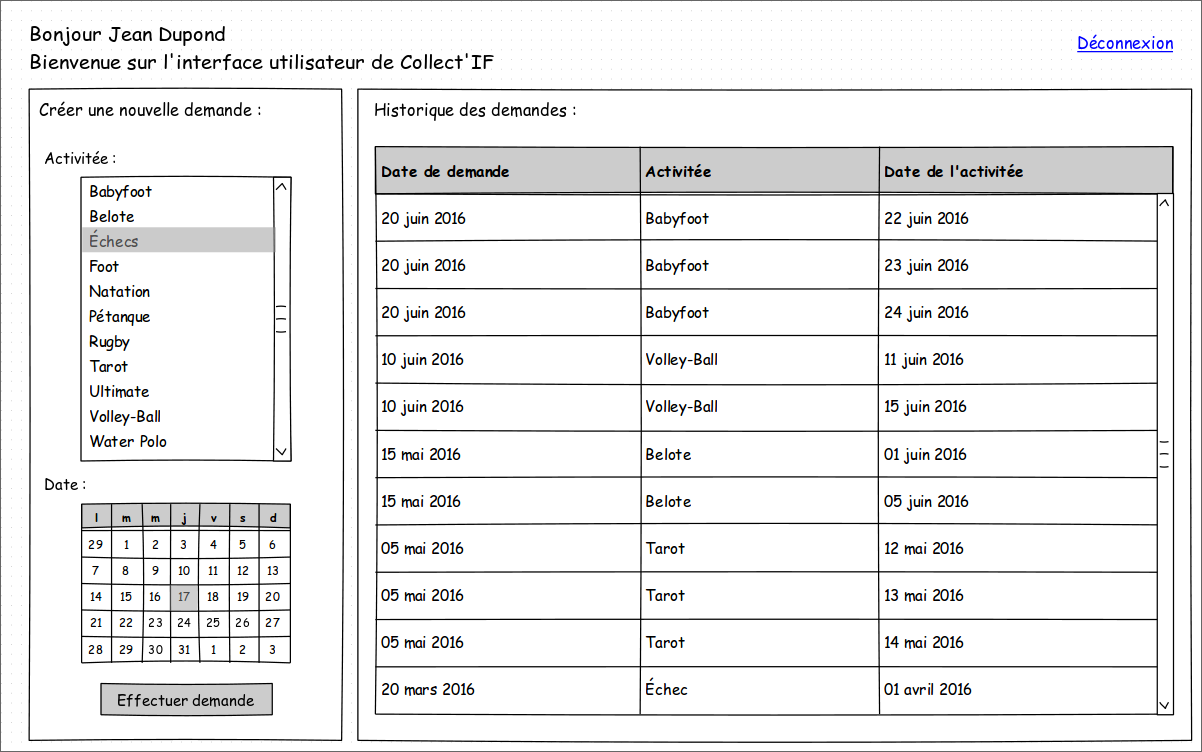
\includegraphics[width=15cm]{../../IHM/IHM_utilisateur.png}
    \caption{IHM utilisateur connecté}
  \end{center}
\end{figure}

\pagebreak
\subsection{IHM Administrateur}

\paragraph{}
L'IHM du responsable est composer de deux colonnes pricipales dont la première est remplie par une liste des évènements affichant la date et le type d'activitée concerné. La segonde colonne est quant à elle desiné à afficher les détail de l'évènement, sélectionner dans la liste de la première colonne, au respossable affin de l'aider dans sont choix. Cette vue est ainsi composé d'un rapelle de la date et de l'activitée concernée ainsi que d'une carte affichant les positions géographique des logement des différents demandeur pour l'évènement. Cette carte affiche de plus les différents lieux qui peuvent être affecté pour l'évènement. Le lieu peut à affecter à l'évènement peut ensuite être choisi soit en selectionnant directement sur la carte ou bien en utilisant le menu déroulant endesous, ce menu étant équiper d'un fonction de recherche permétant d'accéder rapidment à un lieu connu par le responsable.

L'IHM du responsable n'étant accesible que depuis un lieu particulier il n'est pas nécésaire d'avoir une interface de connexion et déconnexion.

\begin{figure}[H]
  \begin{center}
    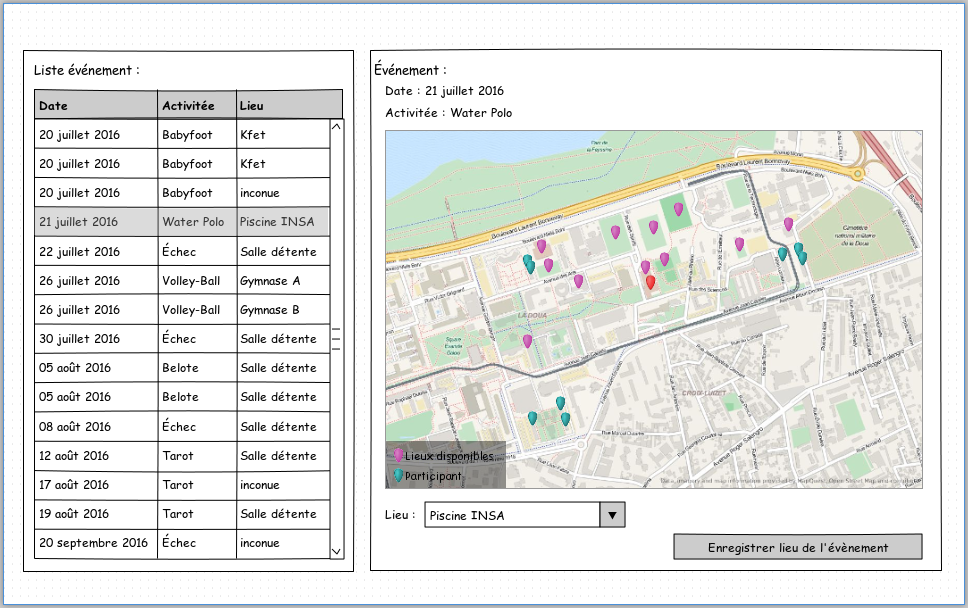
\includegraphics[width=15cm]{../../IHM/IHM_responsable.png}
    \caption{IHM Administrateur}
  \end{center}
\end{figure}



\end{document}

